\section{Квантовые корреляции}

\subsection{Парадокс Эйнштейна — Подольского — Розена}
% Важным этапом в истории развития квантовой теории является объяснение корпускулярно-волнового дуализма.

\subsubsection{Историческая справка}

Важнейший вклад в развитие корпускулярной теории света был сделан Исааком Ньютоном.
В 1704 году им был опубликован трактат ``Оптика'',
в котором рассматриваются фундаментальные законы,
касающиеся прохождения света при преломлении через призмы и линзы, дифракция, интерференция.
Несмотря на сложности, связанные с описанием дифракции в рамках корпускулярной теории, которой он посвятил вторую и третью часть своего трактата,
Ньютон оставался ярким сторонником корпускулярной теории.
Его работа впоследствии определила основные пути развития оптики.

В 1815 году Огюстен Жан Френель дополнил принцип Христиана Гюйгенса,
описывающий механизм распространения вторичных волн,
введя представления о когерентности и интерференции элементарных волн.
Данный результат позволил легко объяснить явление дифракции
и поставил под сомнение корпускулярную теорию света,
которая на тот момент оставалась главенствующей.
В 1818 году сторонник корпускулярной теории Симеон Дени Пуассон
в рамках волновой теории доказал теоретически существование яркого пятна,
возникающего за непрозрачным телом,
освещённым направленным пучком света,
в области его геометрической тени.
Абсурдность результата предполагалось использовать как аргумент против принципа Гюгенса-Френеля,
однако Доминик Араго поставил этот эксперимент.
Результаты эксперимента подтвердили предсказание,
а пятно Пуассона оказалось весомым аргументом в пользу новой волновой теории.

В 1873 году Джеймс Клерк Максвелл в знаменитом «Трактате об электричестве и магнетизме»
привел математическую форму для описания эффекта электромагнитной индукции,
открытого Майклом Фарадеем в 1831 году.
Из полученных Максвеллом уравнений для напряженности магнитного поля вытекало, что в пустом пространстве может распространяться электромагнитная волна, и что её скорость равна скорости света.
Эти рассуждения позволили Максвеллу сделал вывод об электромагнитной природе света.
В 1888 году в свет вышла фундаментальная работа Генриха Рудольфа Герца «Об электродинамических волнах в воздухе и их отражении»,
которая подтвердила гипотезу Максвелла.

В 1900 лорд Рэлей на основе теоремы о равнораспределении энергии по степеням свободы
получил закон распределения энергии излучения в спектре абсолютно чёрного тела в зависимости от температуры.
Закон Рэлея — Джинса правильно описывал низкочастотную часть спектра,
но при средних и высоких частотах приводил к резкому расхождению с экспериментом.
Решение ``ультрафиолетовой катастрофы'' предложил Макс Планк.
Предположив, что энергия изменяется порциями, то есть квантуется,
им был получен закон, который достоверно описывал спектральную плотность излучения абсолютно чёрным телом.

В 1902 году Филипп Ленард на основе результатов экспериментов по фотоэффекту заключил,
что, вопреки волновой теории света,
энергия вылетающего электрона всегда строго связана с частотой падающего излучения и практически не зависит от интенсивности облучения.
В 1905 году Альберт Эйнштейн объяснил теорию фотоэффекта, основываясь на гипотезе Макса Планка о квантовании энергии.
В своей работе Альберт Эйнштейн постулировал,
что с электронами в веществе взаимодействуют отдельные кванты света,
обладающие свойствами частиц.
В последующих своих работах Эйнштейн подчеркивал важность применения принципа корпускулярно-волнового дуализма.
В 1926 году химик Гилберт Льюис ввел термин для кванта света --- ``фотон''.

В 1923 году Луи де Бройль, развивая представления о двойственной корпуску\-лярно-волновой природе света,
выдвинул гипотезу об универсальности корпуску\-лярно-волнового дуализма.
Он утверждал, что не только фотоны, но и электроны и любые другие частицы материи наряду с корпускулярными обладают также волновыми свойствами.
Вскоре Джордж Томсон и Клинтон Джозеф Дэвиссон с Лестером Джермером независимо обнаружили дифракцию электронов, дав тем самым убедительное подтверждение реальности волновых свойств электрона и правильности квантовой механики.

В 1927 году Вернером Гейзенбергом был сформулирован принцип, устанавливающий предел точности одновременного определения пары характеризующих систему квантовых наблюдаемых. Этот результат и предположение Макса Борна о том,
что законы квантовой механики оперируют с вероятностями событий,
легли в основу Копенгагенской интерпретации квантовой механики.

В 1935 году группой авторов во главе с Альбертом Эйнштейном был предложен мысленный эксперимент,
демонстрирующий нарушение принципа неопределенности Гейзенберга.
Впоследствии этот эксперимент получит название ``ЭПР-парадокс''.
В том же году Эрвин Шредингер поддержал Эйнштейна
и опубликовал мысленный эксперимент,
который в настоящее время известен как ``Кот Шрёдингера''.

%В последствии вероятностный исход измерения квантового состояния будет обыгран Щредингером. Он предложит мысленный эксперимент для наглядного противоречия вероятностной модели квантовой механики.
%Сегодня этот эксперимент является извейстнейшей демонстрации реального устройства измерения суперпозициии квантовых состояний.

\subsubsection{Нарушение принципа локального реализма}
Работа Эйнштейна -- Подольского -- Розена\cite{Einstein1935}
указывала на неполноту квантовой механики с помощью мысленного эксперимента,
заключающегося в измерении параметров микрообъекта косвенным образом,
без непосредственного воздействия на этот объект.

Допустим, что в определенный момент времени рождается пара фотонов $A$ и $B$,
движущихся в противоположном направлении,
с общей нулевой поляризацией.
Согласно Копенгагенской теории до измерения поляризация фотонов не определена.
Пара фотонов находится в когерентном состоянии $\ket{\Psi}$,
которое является суперпозицией двух возможных состояний:
\begin{equation}\label{eq:entangled-state}
  \ket{\Psi} = \dfrac{
    \ket{\curvearrowright_A \curvearrowleft_B}
    + \ket{\curvearrowleft_A \curvearrowright_B}
  }{\sqrt{2}}.
\end{equation}
Если теперь измерить состояние одного из фотонов,
то второй фотон,
как бы далеко он ни был,
мгновенно подстроится.
Состояние второго фотона будет определенным.
В своей работе\cite{Einstein1935} авторы заключают,
что из Копенгагенской теории следует,
что существует дальнодействующее взаимодействие между фотонами,
распространяющееся быстрее скорости света.

Этот мысленный эксперимент долгое время был аргументом
в пользу теории скрытых параметров.
Эйнштейн был уверен,
что никакой неопределенности нет,
и что фотоны на самом деле всегда имеют детерминированную поляризацию.
В 1964 году Джон Стюарт Белл сформулировал неравенства\cite{Bell1964},
проверяющие,
что введение дополнительных параметров не может сделать описание квантовой механики детерминированным.
Неравенство Белла показывает,
что определенные статистические корреляции,
предсказываемые квантовой механикой для измерений на двухчастичных ансамблях,
не могут быть поняты в рамках реалистической картины,
основанной на локальном реализме\cite{Einstein1935}.

В 70-е годы были проведены первые эксперименты\cite{Alain1976} Джоном Клаузером и Аленом Аспе для проверки неравенств Белла,
а в 2008 году был проведен комплексный эксперимент\cite{Scheidl2010},
который окончательно подтвердил нелокальный характер квантовой теории.

В 2010 году Джон Клаузер, Ален Аспе и Антон Цайлингер стали лауреатами премии Вольфа по физике ``за фундаментальный концептуальный и экспериментальный вклад в основы квантовой физики, в частности, за серию возрастающих по сложности проверок неравенств Белла с использованием запутанных квантовых состояний''.

В действительности  ЭПР-парадокс не является парадоксом,
а, скорее, примером контринтуитивной природы квантовой механики.
При измерении фотона $A$ в состоянии~(\ref{eq:entangled-state}),
несмотря на то, что состояние фотона $B$ становится детерминированным,
передачи информации не происходит.
Наблюдатель фотона $B$ не будет знать его поляризацию,
не произведя измерения.
Однако результат его измерения будет детерминированным,
и может быть предсказан наблюдателем измеренного фотона $A$.

В современной науке состояния типа~(\ref{eq:entangled-state}) называются запутанными состояниями, а также состояниями Белла.


\subsection{Многочастичная запутанность}
% Phys. Rev. A 85, 022321 (2012)  B. Multiparticle Entanglement

%We give now a definition of many-particle entanglement  \cite{fisher_and_entanglement}.
%A pure state is $k$-particle entangled, if it can be written as a product \mbox{$\left| \Psi_\mathrm{k-ent} \right\rangle = \otimes^M_{l=1} \left| \Psi_l \right\rangle$}, where $\left| \Psi_l \right\rangle$ is a state of $N_l$ particles \mbox{($\sum\limits_{l=1}^M N_l = N$)}, each  $\left| \Psi_l \right\rangle$ does not factorize, and the maximal $N_l \geq k$. A generalisation for mixed states is straightforward \cite{fisher_and_entanglement}.

% Многочастичная запутанность не имеет строгого определения.
В данной работе сделан акцент на количественную оценку числа запутанных частиц в системе,
поэтому удобно следовать классификации из работ~\cite{Seevinck2001, Toth2005, Bancal2009, Chen2005, Guhne2005, Guhne2006}.
Существуют альтернативные~\cite{Dur1999, Dur2000} способы классификации запутанности,
но в данной работе они рассмотрены не будут.

\begin{definition}\label{def:manyparticle-entanglement}
  Чистое состояние $N$ частиц является $k$-частино запутанным, если
  $$
  \left| \Psi_{k-\mathrm{ent}} \right\rangle
  	= \otimes^\mathrm{M}_{i=1} \left| \Psi_{i} \right\rangle,
  $$
  где $\left| \Psi_{i} \right\rangle$ - это многокубитное несепарабельное или однокубитное состояние подсистемы с $N_i$ частицами
  $\left( \sum_{i=1}^N N_i = N \right)$,
  и существует такое  $ m \in \mathbb{N}$, что $N_{m} \ge k$.
  Смешанное состояние $\rho_{k-\mathrm{ent}}$ может быть представлено как
  $$
  \rho_{k-\mathrm{ent}} =
  \sum\limits_{l} p_l \ket{\Psi_{k_l-\mathrm{ent}}}\bra{\Psi_{k_l-\mathrm{ent}}},
  $$
  где $k_l \geq k$ для любого $l$.
\end{definition}


Проиллюстрируем классификацию многочастичной запутанности на примере системы из $N = 3$ частиц.
Состояние
$\ket{\Psi_\mathrm{no-ent}} = \ket{\varphi}_1 \otimes \ket{\phi}_2 \otimes \ket{\chi}_3$
является полностью сепарабельным.
Состояние
$\ket{\Psi_{2-\mathrm{ent}}} = \ket{\varphi}_{12} \otimes \ket{\chi}_3$
является двухчастично запутанным,
так как $\ket{\varphi}_{12}$ не факторизуется
$\ket{\varphi}_{12} \neq \ket{\varphi}_1 \otimes \ket{\phi}_2$.
Несепарабельное состояние $\ket{\Psi_{3-\mathrm{ent}}}$ является трехчастично запутанным.


\subsection{Методы детектирования запутанных состояний}
\label{sec:entanglement-criteria}
Ввиду широкого распространения запутанности как важного ресурса,
естественно, возникает вопрос о методах детектирования запутанных состояний.
Первый эффективный инструмент,
использующийся для определения запутанных состояний - это неравенства Белла~\cite{Bell1964}.
Существуют различные неравенства типа Белла, используемые для обнаружения запутанных состояний~\cite{Collins2002, Seevinck2001, Toth2005, Nagata2002, Yu2003, Laskowski2005, Schmid2008, Bancal2009, Svetlichny1987, Gisin1998}.
Например, для некоторого набора спиновых наблюдаемых можно воспользоваться теоремой Гисина~\cite{Gisin1991},
которая утверждает, что
все запутанные двухквантовые чистые состояния нарушают неравенство Клаузера-Хорна-Шимони-Холта~\cite{Clauser1969}.
Наиболее простым критерием бинарной запутанности чистого состояния $\psi$ подсистем А и B является энтропия фон Неймана
%
\begin{equation}
  S^\mathrm{A} = - \tr{\rho^\mathrm{A} \log_2 \rho^\mathrm{A}},
\end{equation}
%
где $\rho^\mathrm{A}$ матрица плотности редуцированная по подсистеме B
\begin{equation}
  \rho^\mathrm{A} = \tr{\psi}_\mathrm{B}.
\end{equation}
Если эта энтропия равна нулю, то состояние $\psi$ не запутанно~\cite{Bennett1996}.
Для проверки смешанного состояния $\rho = \sum_i p_i \psi_i$ мера запутанности может быть определена как
\begin{equation}
  E(\rho) = \min\limits_{E} \sum\limits_i p_i S(\psi_i),
\end{equation}
где $S(\psi_i)$ --- энтропия редуцированного чистого состояния $\psi_i$,
а минимум берется по ансамблю $E(\rho) = \left\{p_i, \ket{\psi_i}\right\}$,
который определяет матрицу плотности.

\begin{figure}[H]
    \centering
    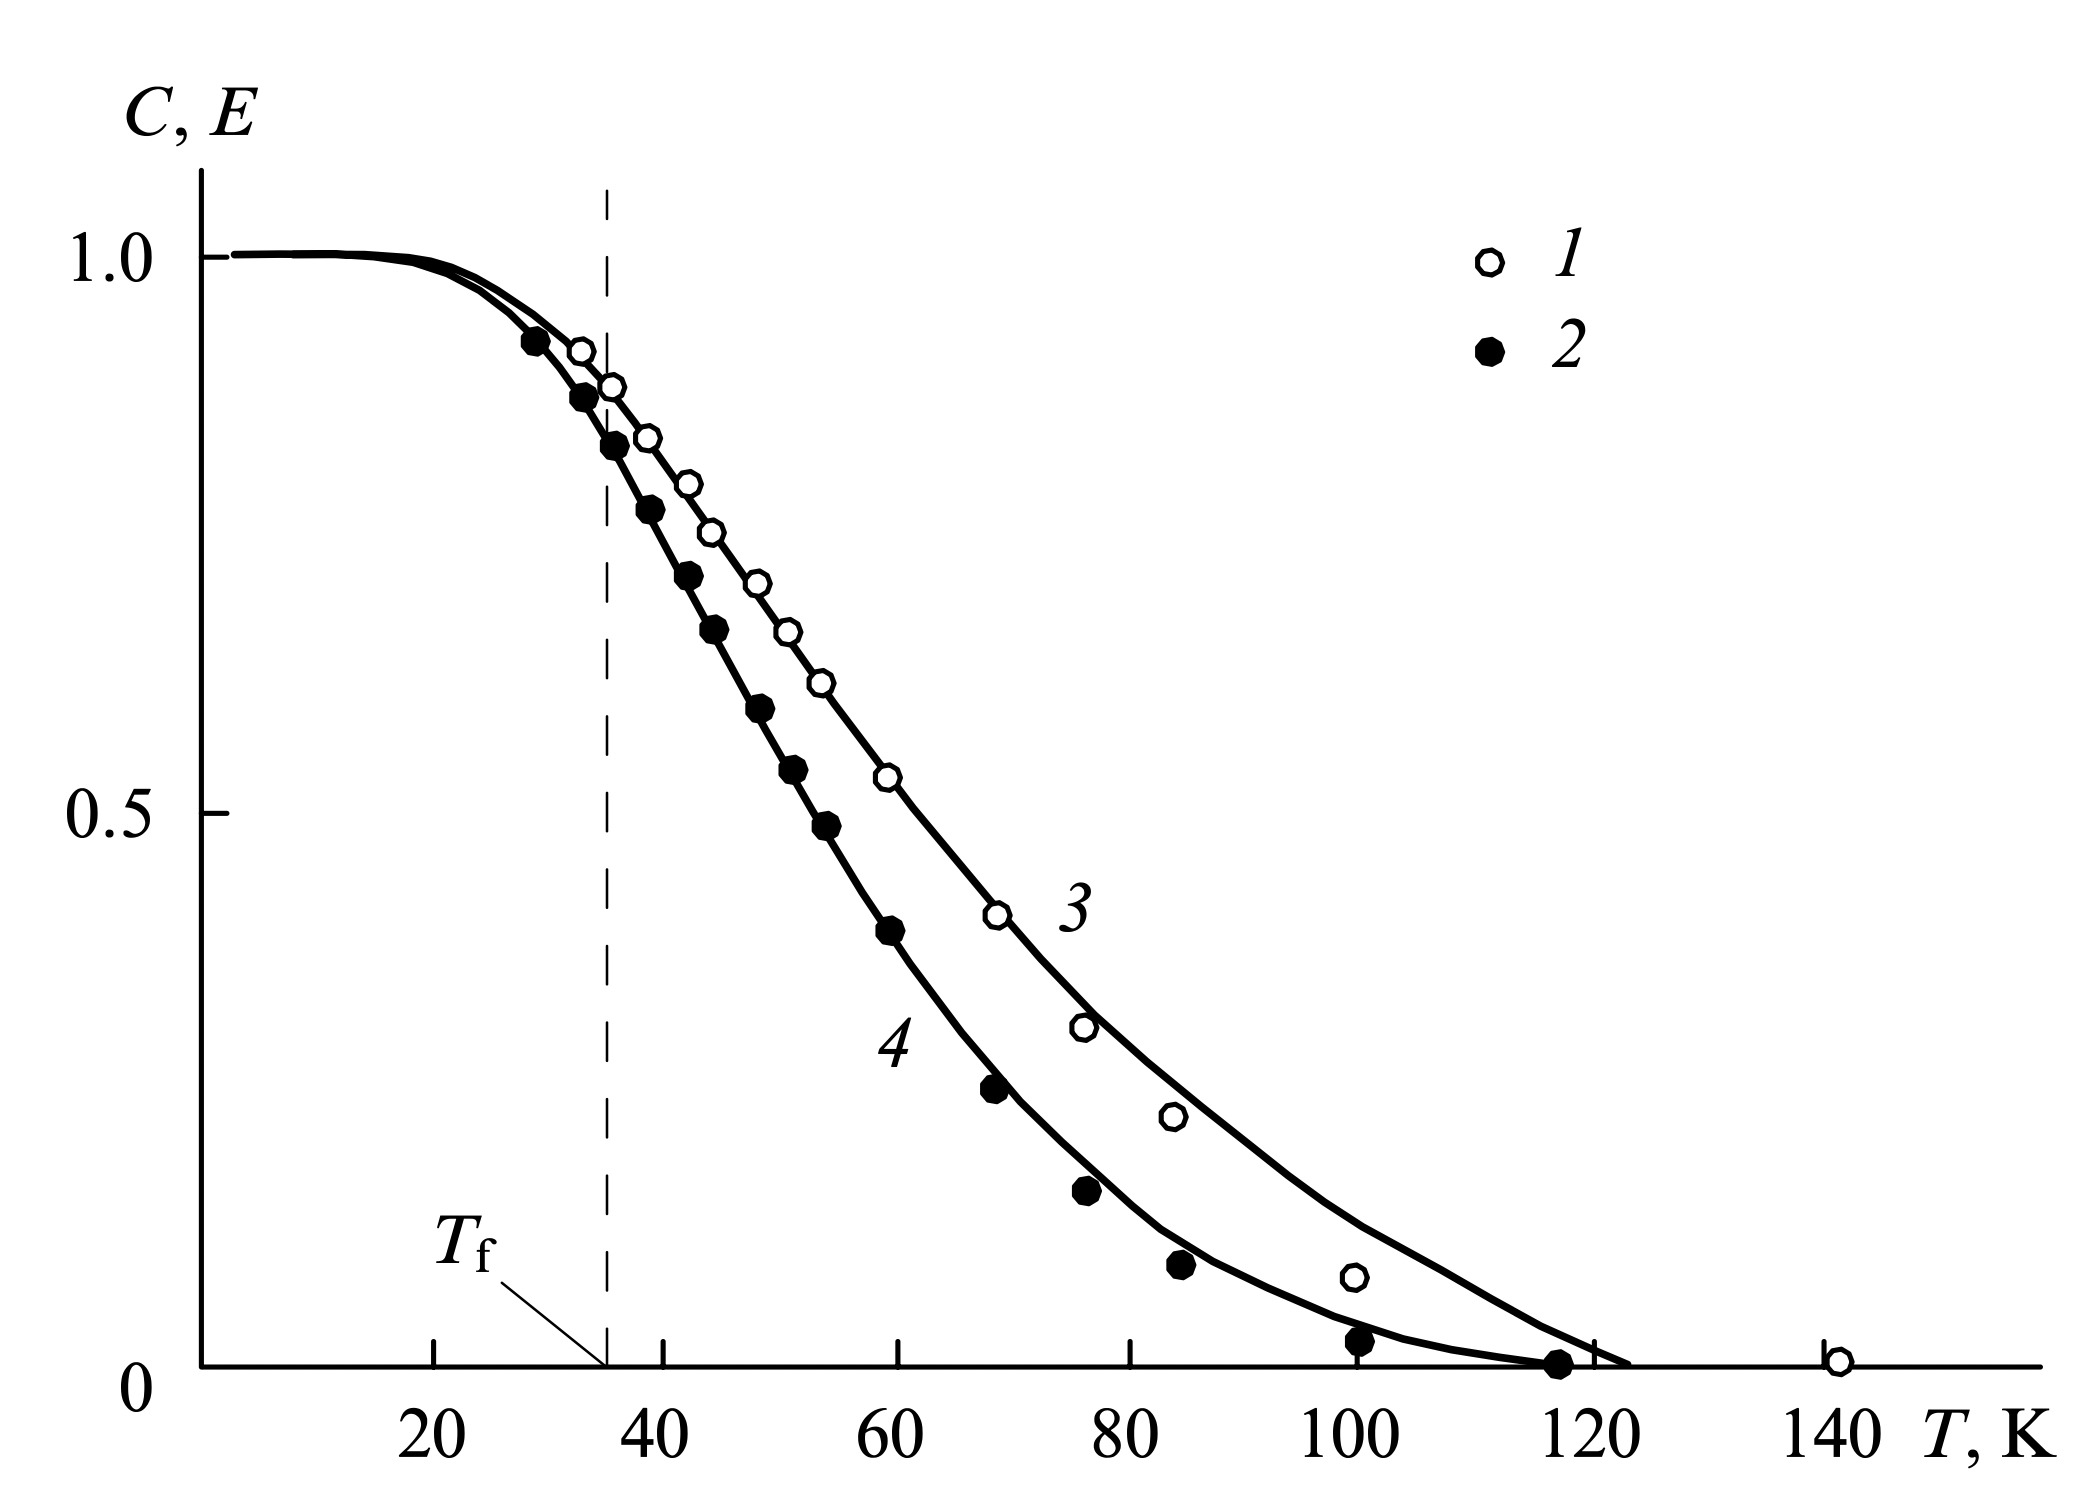
\includegraphics[width=0.5\textwidth]{concurence-temp-rcr}
    \caption{
      Температурные зависимости согласованности (1) и запутанности (2) в     нитрозильном комплексе железа.
      Сплошные кривые 3 и 4 --- теоретические зависимости $C$ и $E$ соответственно.
    }
    \label{fig:concurence-temp-rcr}
\end{figure}

Позднее были разработаны свидетели запутанности~\cite{Wootters1998, Bourennane2004, Kaszlikowski2008, Krammer2009, Bancal2011},
например, согласованность Вуттерса,
% Phys. Rev. A 85, 022321 (2012) Intorduction
а также критерии на основе неравенств ``сжимания'' спинов (spin-squeezing)~\cite{Sorensen2001, Durkin2005, Vitagliano2011, Duan2011}.
Согласованность является очень популярной мерой для количественной оценки двучастичных квантовых корреляций.
Она может быть определена как для чистых состояний,
так и для смешанных.
Вуттерс~\cite{Wootters1998} показал, что
%
\begin{equation}\label{eq:concurrence}
  C(\rho)
  = \max\left\{0, \lambda_1 - \lambda_2  - \lambda_3  - \lambda_4\right\}.
\end{equation}
%
Здесь $\lambda_1 \geq \lambda_2 \geq \lambda_3 \geq \lambda_4$ --- собственные числа матрицы
%
\begin{equation}
  R = \sqrt{\sqrt{\rho}\tilde{\rho}\sqrt{\rho}},
\end{equation}
где
%
\begin{equation}
  \tilde\rho = \p{\sigma_y \otimes \sigma_y}
    \rho^* \p{\sigma_y \otimes \sigma_y}.
\end{equation}
%
Также в общем случае смешанных двухкубитных систем запутанность $E(\rho)$ является функцией согласованности
\begin{equation}
  E(\rho) = H\p{\dfrac{1 + \sqrt{1 - C^2}}{2}},
\end{equation}
%
где $H(x)$ --- функция Шеннона~\cite{Shannon1948}
%
\begin{equation}
  H(x) = -x \log_2 x - (1 - x)\log_2(1 - x).
\end{equation}
%
Популярность критерия Вуттерса объясняется тем,
что выражение~(\ref{eq:concurrence}) может быть получено в аналитической форме.
В случае двухкубитной матрицы плотности, обладающей блочно-диагональной структурой вида
%
\begin{equation}
  \rho = \begin{pmatrix}
    u &  0  &  0  & 0 \\
    0 & x_1 &  w  & 0 \\
    0 &  w* & x_2 & 0 \\
    0 &  0  &  0  & v
  \end{pmatrix},
\end{equation}
%
согласованность определяется простой формулой:
%
\begin{equation}
  C = 2 \max\left\{0, |w| - \sqrt{uv} \right\}.
\end{equation}
%
В результате появляется возможность связать согласованность с реальными наблюдаемыми величинами.
Например, в работе~\cite{Aldoshin2012} была исследована температурная зависимость согласованности
в димере нитрозильного комплекса железа на основе магнитной восприимчивости антиферромагнитного димера (см. Рис.~\ref{fig:concurence-temp-rcr}).

Недавно другие подходы привели к критериям, которые могут быть оценены непосредственно по элементам матрицы плотности~\cite{Guhne2010, Huber2010}.
Дальнейшие работы по обнаружению многочастичного запутывания можно найти в работах~\cite{Li2010, Jungnitsch2011, Vicente2011, Huber2011} и в обзоре~\cite{Guhne2009}.
В частности, квадратичные неравенства типа Белла были получены Уффинком~\cite{Uffink2002} в качестве тестов на многочастичную запутанность
и используются для классификации всех состояний $N$~кубитов на $N-1$~классов запутанности от двухчастично запутанного и до полностью запутанного
 ($N$-запутанного) состояния~\cite{Yu2003}.
Критерий на основе энтропии Реньи~\cite{Hosur2016, Fan2017}
является строгим свидетелем многочастичной запутанности для чистых состояний.
Энтропия Реньи может быть измерена экспериментально,
но для этого требуются ресурсы,
которые экспоненциально масштабируются с размером изучаемой системы,
а также возможность одночастичной адресации.

Хотя существуют и некоторые другие меры запутанных состояний, проблема классификации и количественного измерения
запутанности в целом всё ещё далека от полного
понимания~\cite{Guhne2009}.


\subsubsection{Оценка количества запутанных частиц в системе}
\label{sec:manyparticle-entanglement-criteria}
% Phys. Rev. A 85, 022321 (2012)  B. Multiparticle Entanglement
В то время как структура множества запутанных двучастичных квантовых состояний достаточно хорошо изучена,
о классификации и количественной оценке запутанности многочастичных квантовых состояний известно меньше\cite{Plenio2007, Amico2008, Horodecki2009, Guhne2009}.
%
В данной работе будет подробно рассмотрен критерий,
использующий  неравенства Белла\cite{Bell1964} в терминах обобщенной меры информации $F$.

\begin{definition}\label{def:f}
Обобщенной мерой информации называется такая функция $F$,
которая удовлетворяет следующим свойствам:
\begin{enumerate}
  \item Значение меры объединения двух независимых подсистем --- это сумма значений меры, вычисленной для каждой подсистемы индивидуально:
  \begin{equation}\label{eq:f-additive-map}
    F(\rho_1 \otimes \rho_2 ,H_1 \otimes I_2 + I_1 \otimes H_2)
    = F_{1} (\rho_1, H_1) + F_{2} (\rho_2 , H_2),
  \end{equation}
  где $H_i$ --- это оператор, действующий на подсистему $\rho_i$,
  а $I_i$ --- это единичный оператор.

  \item Известна верхняя граница величины меры для системы $N$ частиц:
  \begin{equation}\label{eq:f-supremum}
    F \leq N^2.
  \end{equation}
\end{enumerate}
\end{definition}

\begin{definition}\label{def:rho-k-prod}
  Матрица плотности $\rho_{k-\mathrm{prod}}$
  является $k$-частично разделимой,
  если она может быть факторизована на $l$ подсистем $\{\rho_i\}$ с размерами $\{N_i\}$,
  где $\rho_i$ --- несепарабельное многокубитное состояние или однокубитное состояние,
  и выполнено неравенство
  \begin{equation}
    N > k \geq N_1 \geq N_2 \geq \dots \geq N_l \geq 1,
    \quad
    \sum_{i=0}^{l} N_i = N.
  \end{equation}
\end{definition}
%
% Из свойств обобщенной меры информации $F$ следует,
% что для множества состояний $\mathcal{N} = \left\{\rho_{k-\mathrm{prod}}\right\}$ системы $N$ частиц%,
% % в которых максимальный размер несепарабельной подсистемы равен $k < N$,
% оценку (см. свойство \ref{eq:f-supremum}) ее верхней границы можно улучшить.
% Рассмотрим некоторое состояние $\rho_{k-\mathrm{prod}} \in \mathcal{N}$ ,
% которое может быть факторизованно на $l$ подсистем $\{\rho_i\}$,
% являющихся несепарабельными многокубитными состояниями или однокубитными состояниями, с размерами $\{N_i\}$, так что:
% \begin{equation}
%   N > k \geq N_1 \geq N_2 \geq \dots \geq N_l \geq 1,
%   \quad
%   \sum_{i=0}^{l} N_i = N.
% \end{equation}
%
Из свойств обобщенной меры информации $F$ следует,
что для произвольной $k$-частично разделимой матрицы плотности $\rho_{k-\mathrm{prod}}$~(см.~определение~\ref{def:rho-k-prod})
% что для множества состояний $\mathcal{N} = \left\{\rho_{k-\mathrm{prod}}\right\}$
% системы $N$ частиц,
оценку~(см.~свойство~\ref{eq:f-supremum}) ее верхней границы можно улучшить.
Используя свойство аддитивности~(\ref{eq:f-additive-map}) меры $F$,
можно оценить сверху величину обобщённой информации для каждой подсистемы отдельно
%
\begin{equation}\label{eq:f-subsystems}
  F(\rho_{k-\mathrm{prod}}) =
  F(\rho_1) + F(\rho_2) + \dots + F(\rho_l)
  \leq N^2_1 + N^2_2 + \dots + N^2_l.
\end{equation}
%
Максимальное значение правой части выражения~(\ref{eq:f-subsystems}) достигается,
когда система состоит из $m = \left[\frac N k \right]$ подсистем размера $k$
и одной подсистемой с остатком
%
\begin{equation}\label{eq:f-worse-distribution}
  \sup_{\left\{\rho_{k-\mathrm{prod}}\right\}}
    \left(N^2_1 + N^2_2 + \dots + N^2_l\right)
  = \underbrace{
    k^2 + k^2 + \dots + k^2
    }_{m = \left[\frac N k \right] \, \mbox{раз}}
    + \underbrace{(N-km)^2}_{\mbox{остаток}}.
\end{equation}
%
Докажем это утверждение.
Рассмотрим два последних слагаемых выражения~(\ref{eq:f-worse-distribution}) и предположим, что
%
\begin{multline}\label{eq:n-i-distribution-inequality}
  k^2 + (N-km)^2 < (k - 1)^2 + (N-km + 1)^2 \\
  = k^2 + (N-km)^2
    - 2\p{k - 1 \underbrace{(N-km)}_{ = \phi, \, 0 \leq \phi < 1}} \\
  = k^2 + (N-km)^2 - 2(k - 1 - \phi).
\end{multline}
%
Неравенство~(\ref{eq:n-i-distribution-inequality}) нарушается при $k \geq 2$. Противоречие.
Правая часть выражения~(\ref{eq:f-entangled}) не превосходит $N^2$.
С учетом
$m = \left[\frac{N}{k}\right] = \frac{N}{k} -\phi$ ($0 \leq \phi < 1$)
получаем
%
\begin{equation}
  k^2m + \p{N-km}^2
  = k^2\left(\frac{N}{k} - \phi\right) + (N - N +k\phi)^2  < kN \leq N^2.
\end{equation}
%
Объединяя выражения~(\ref{eq:f-subsystems})~и~(\ref{eq:f-worse-distribution}),
получаем верхнюю границу величины меры $F$ для $k$-разделимой матрицы плотности $\rho_{k-\mathrm{prod}}$ системы $N$
%
\begin{equation}\label{eq:f-entangled}
  F\p{\rho_{k-\mathrm{prod}}}
  \leq F_{N, k-\mathrm{prod}}
  = \left[ \frac N k \right] k^2 + \left(N - k \left[ \frac N k \right]\right)^2.
\end{equation}
%


Для примера ниже приведены значения $F_{N, k-\mathrm{ent}}$
для систем $N = 2, 3, 4, 5$ частиц:
\begin{itemize}
  \item[(1)]
    $F_{2, 1-\mathrm{prod}}= 2$,
    $F_{2, 2-\mathrm{prod}}= 4$;
  \item[(2)]
    $F_{3, 1-\mathrm{prod}}= 3$,
    $F_{3, 2-\mathrm{prod}}= 5$,
    $F_{3, 3-\mathrm{prod}}= 9$;
  \item[(3)]
    $F_{4, 1-\mathrm{prod}}= 4$,
    $F_{4, 2-\mathrm{prod}}= 8$,
    $F_{4, 3-\mathrm{prod}}= 10$,
    $F_{4, 4-\mathrm{prod}}= 16$;
  \item[(4)]
    $F_{5, 1-\mathrm{prod}}= 5$,
    $F_{5, 1-\mathrm{prod}}= 9$,
    $F_{5, 1-\mathrm{prod}}= 13$,
    $F_{5, 1-\mathrm{prod}}= 17$,
    $F_{5, 1-\mathrm{prod}}= 25$.
\end{itemize}


\begin{theorem}\label{th:entanglement-criteria}
  Состояние $\rho$ является $k$-частично запутанным $\rho_\mathrm{k-ent}$,
  если оно удовлетворяет неравенству
  \begin{equation}\label{eq:entanglement-criteria}
    F_{N, (k-1)-\mathrm{prod}} < F(\rho),
  \end{equation}
\end{theorem}
\textbf{Доказательство.}
Пусть $F_{N, (k-1)-\mathrm{prod}} < F(\rho)$ выполнено,
но состояние $\rho$ не является $k$-частично запутанным.
Тогда согласно определению~\ref{def:manyparticle-entanglement} максимально возможный размер несепарабельной подсистемы равен  $k-1$,
и,
согласно определению~\ref{def:rho-k-prod} состояние $\rho$ является $k-1$-частично разделимым.
Согласно выражению~\ref{eq:f-entangled}, величина обобщенной информации $k-1$-частично разделимой матрицы плотности не может превышать $F(\rho) \leq F_{N, (k-1)-\mathrm{prod}}$.
Противоречие.

В настоящее время признано,
что большинство физических процессов в природе можно сформулировать в терминах обработки информации,
и концепция информации может быть центральной для понимания квантовой теории\cite{Wheeler2004, Summhammer2004, Frieden2004}.
В частности, в качестве обобщённой информационной меры в квантовой теории информации могут выступать
\begin{enumerate}
  \item Косая информация Вигнера-Янасе\cite{Zeqian2005},
  \item Квантовая информация Фишера\cite{Hyllus2012}.
\end{enumerate}

% В частности, было показано\cite{Garttner2018},
% что нижняя граница квантовой информации Фишера соответствует
% второму моменту спектра интенсивностей многоквантовых когерентностей.